\documentclass[10pt,twocolumn,letterpaper]{article}

\usepackage{cvpr}
\usepackage{times}
\usepackage{epsfig}
\usepackage{graphicx}
\usepackage{amsmath}
\usepackage{amssymb}
\usepackage{makecell}
\usepackage{booktabs}

% Include other packages here, before hyperref.

% If you comment hyperref and then uncomment it, you should delete
% egpaper.aux before re-running latex.  (Or just hit 'q' on the first latex
% run, let it finish, and you should be clear).
\usepackage[breaklinks=true,bookmarks=false]{hyperref}

\cvprfinalcopy % *** Uncomment this line for the final submission

\def\cvprPaperID{****} % *** Enter the CVPR Paper ID here
\def\httilde{\mbox{\tt\raisebox{-.5ex}{\symbol{126}}}}

\usepackage{caption} 
\captionsetup[table]{skip=10pt}

% Pages are numbered in submission mode, and unnumbered in camera-ready
%\ifcvprfinal\pagestyle{empty}\fi
\setcounter{page}{4321}
\begin{document}

%%%%%%%%% TITLE
\title{Video Compression with 3D Convolutional Neural Networks}

\author{Brennan Shacklett\\
Stanford University\\
Stanford, CA\\
{\tt\small bps@cs.stanford.edu}
% For a paper whose authors are all at the same institution,
% omit the following lines up until the closing ``}''.
% Additional authors and addresses can be added with ``\and'',
% just like the second author.
% To save space, use either the email address or home page, not both
}

\maketitle
%\thispagestyle{empty}

%%%%%%%%% ABSTRACT
\begin{abstract}
  Video compression is an increasingly important area of research due to demands from online streaming applications. Conventional lossy compression algorithms exploit both spatial and temporal redundancy within videos to achieve large compression savings; however, these algorithms are the product of extensive fine tuning and careful approximations, which can make further innovation difficult. Rather than a conventional video compression scheme, this work uses a 3D Convolutional Neural Network combined with an autoencoded residual to learn the relationship between sections of video and generate a prediction of the next frame. Only the autoencoder's internal representation is necessary to decode videos in this scheme, which enables considerable compression savings with relatively little distortion on many scenes as measured by MS-SSIM, particularly in low bitrate contexts.
\end{abstract}

%%%%%%%%% BODY TEXT
\section{Introduction}

As the resolution and framerate demands of both viewers and content creators increase, the bandwidth and computation demands of online video streaming continue to grow. While transferring raw video data is impractical due to massive bandwidth requirements, in a typical video the current frame is closely correlated with the previous frame, since generally the camera and scene will only have moved slightly in the interval between frames. Modern lossy video compression algorithms are able to exploit this temporal redundancy to achieve considerable compression savings with minimal distortion.

Current video codecs are the product of many years of fine tuning and careful approximations, which can make development of innovative new techniques difficult without breaking the finely tuned balance of a wide variety of different codec features. Additionally, in modern codecs, compression savings have come at the cost of ever increasing computational demands: AV1, a state of the art codec achieves around 50\% compression savings when compared to VP9 (a previous gen codec), but this comes at the cost of 4-10 times the encoding complexity \cite{netflix}.

One important note is that despite this increasing computational complexity, these codecs do not attempt to make ``intelligent'' predictions of the next frame based on the current frame's visual information. Instead, codecs contain a large library of different prediction modes, which each perform a relatively simple prediction such as copying pixels from one block of video to another. The optimal mode is then selected by the encoder and transmitted to the decoder as part of the compressed video: therefore most of the complexity in modern video encoders --- both from a design and a computation standpoint --- comes from intelligently selecting the optimal mode for each section of video.

Given the success of neural networks in interpreting visual data and generating new visual data, it seems natural that neural networks should be able to improve upon the techniques used in conventional video codecs. Furthermore, the automatic nature of neural network optimization means that neural network based video encoders should considerably reduce the difficulty of experimenting and innovating in this field, since new network structures can be quickly optimized and tested when compared to the painstaking process of developing a new feature in a conventional codec.

This work explores one of many possible directions for neural network based video compression: using convolutional neural networks to predict the next frame in a video sequence based on previous frames, combined with autoencoder based compression of the residual between the predicted frame and the true frame. In this scheme, a given frame in a video sequence is reconstructed by first using a CNN to predict the current frame based on a set number of previous frames, and then decoding the compressed residual and adding it to the prediction. Therefore the complete network takes in the previous $N$ frames along with the current frame as input, and produces a single image --- the reconstruction --- along with the compressed residual.

\section{Related Work}
Although there is extensive literature in the field of conventional video compression, little of it is particularly useful to this work, which aims to build a purely neural network based compression approach. While combining conventional techniques with small neural network based components can be successful as shown by Chen et al \cite{av1improv1} and Fu et al \cite{av1improv2} in their work on adding prediction modes to AV1, such approaches still suffer from the difficulties of choosing features and prediction modes found in conventional codec development. The original paper describing the MPEG codec \cite{LeGall} provides a good reference for the basic techniques still employed by most conventional video codecs, which can be seen as a baseline for the types of features a neural network based approach needs to emulate in order to be successful. For the purposes of this project, the key emulated features are prediction from previous frames and compression of the residual. One key component of traditional compression is probalistic entropy coding as the final step of compression in order to ensure as dense a binary representation as possible; however for simplicity this was not explored in the project.

In recent years, there has been growing interest in applying neural networks to compression problems, but thus far most work has focused on single image compression rather than video. Two relatively recent papers from Wu et al \cite{DBLP:journals/corr/abs-1804-06919} and Chen et al \cite{DBLP:journals/corr/abs-1804-09869} describe deep learning based video compression schemes, but both require external motion estimation algorithms rather than learning motion prediction in the network. Since motion prediction --- the process of predicting where pixels from previous frames should be placed in the next frame --- is the key source of removing temporal redundancy in video compression, this project aimed to avoid offloading this step to a external algorithm. Instead, inspired by the success of 3D CNNs for video action recognition and segmentation \cite{DBLP:journals/corr/abs-1712-01111}, as well as the use of 3D CNNs for image sequence block matching and denoising \cite{DBLP:journals/corr/AhnC17}, this project relies on 3D CNNs to perform motion prediction.

Both Wu et al and Chen et al also rely on dividing the video into a series of fixed size blocks rather than operating on entire frames, which allows deeper networks to be possible without unrealistic computation demands. This approach is also used extensively in conventional video compression, where each frame is divided into spatially correlated blocks and subblocks to allow many different prediction modes in the same frame. Due to the success of dividing videos into blocks in these papers as well as in conventional compression, this project also divides the input video into fixed size blocks, which reduces the memory footprint of the networks and effectively increases the amount of training data available.

After the prediction step, these learning based video compression schemes rely on techniques similar to ones used in single image compression in order to compress the remaining information required for reconstruction of a video frame. Work by Toderici et al \cite{DBLP:journals/corr/TodericiVJHMSC16}\cite{DBLP:journals/corr/TodericiOHVMBCS15} on neural network based image compression shows the success of various autoencoder and LSTM based approaches for compressing images in 32 by 32 pixel blocks with variable compression rates. These schemes are able to support variable compression rates by additively encoding the image. Rather than simply allowing one pass through the network for each pixel block, the residual for a given block can be passed back through the network to reduce errors at the cost of less compression. Although Toderici et al's work concludes that using convolutional LSTMs is currently the optimal approach for image compression, this project uses a network based on their convolutional autoencoder structure for compressing the residual, due to its relative simplicity and easier training. Newer work by Minnen et al \cite{Minnen} demonstrates how to extend these schemes to allow variable entropy encoding for each block of an image; however while this would undoubtedly improve the performance of this project, it has to be left as a future extension.

\section{Dataset \& Features}
The core dataset used for this project is the \texttt{objective-2-slow} dataset from the Xiph Foundation \cite{xiph}. This dataset contains 75 raw uncompressed videos ranging in resolution from 360p to 4K, and spanning between 30 and 120 frames. A partner dataset from the Xiph Foundation named \texttt{objective-2-fast} also exists, which contains a subset of the videos from \texttt{objective-2-slow} and is designed for faster testing purposes. For the purposes of this project, the \texttt{objective-2-fast} dataset was divided into four parts, with the first part being the test set and the second part being the validation set, and the 3rd and 4th parts combined into the training set along with all the videos from \texttt{objective-2-slow} (except the videos from objective-2-slow already used in testing or validation). Additionally, the testing dataset was combined with long sequences from the Blender Foundation's Big Buck Bunny and Sintel animated movies \cite{blender}, in order to test the algorithms on much longer videos. The testing and validation sets were then divided into a larger number of short sequences to ensure that each had a relatively wide variety of different clips.

This left approximately 50 videos in the training set, fifteen 30 frame videos in the validation set, and fifteen 30 frame videos in the test set (plus the 2 long sequences in the test set). Although these numbers are quite low, all the tested networks operate on each 32x32 block of pixels in the video independently. Since most of the videos are 4K or 1080p, this means the dataset had a very large number of separate 32x32 blocks (approximately 9000 individual blocks for a single frame of a 4K video) to train and test on. Unfortunately many of these blocks are quite similar, especially in high resolution videos where each block represents a relatively small portion of the scene.

\begin{figure}[t]
\begin{center}
  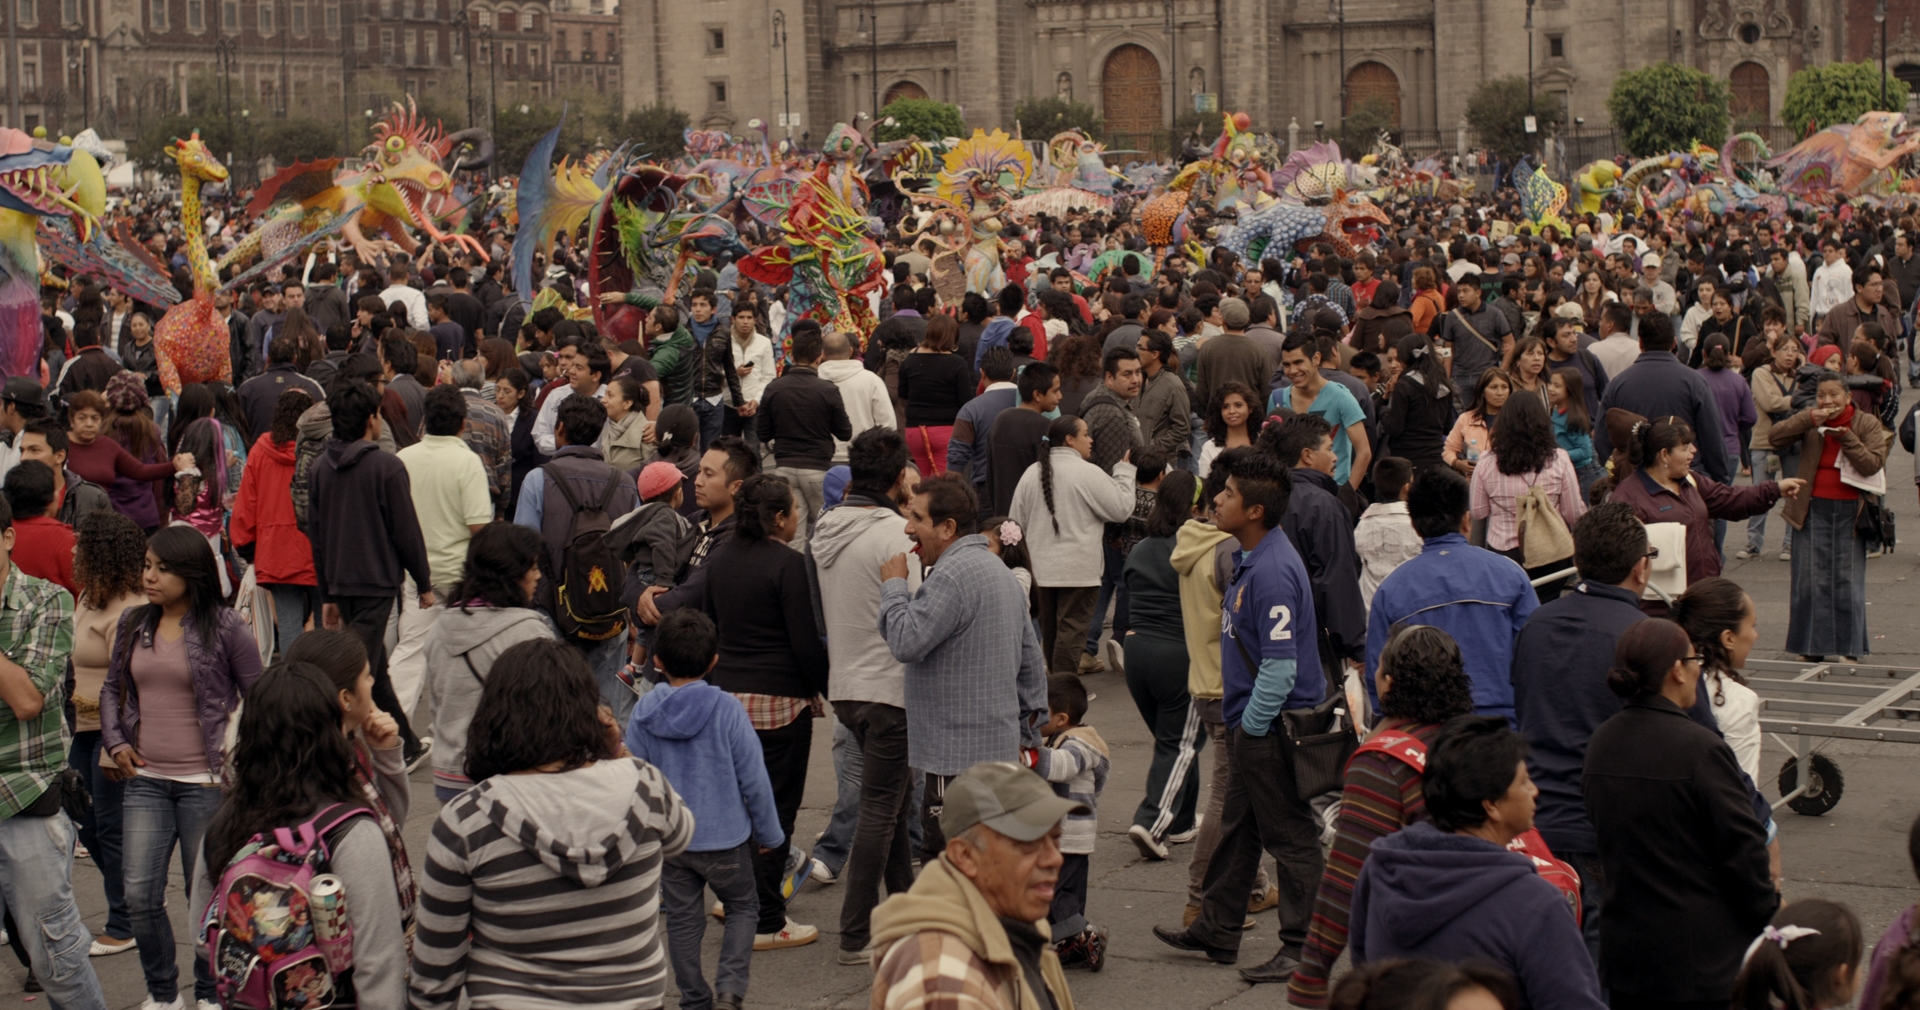
\includegraphics[width=0.8\linewidth]{data_example}
\end{center}
   \caption{Frame from the 1080p ``Netflix\_SquareAndTimelapse'' video from the \texttt{objective-2-slow} dataset.}
\end{figure}

In terms of preprocessing, each video was padded to have both the width and height be multiples of 32, so the network did not have to handle any non square sections of video on the edges; however, this padding was removed for the final distortion metrics on the test set. Additionally the per channel means and standard deviation were computed across the training set for normalization purposes. For efficiency purposes during training, the training set was also transformed to allow stacking multiple independent 32x32 pixel blocks from a given frame together into a single training batch, since different video lengths and sizes made processing different videos in the same batch inefficient. All the source videos were originally stored in YUV 4:2:0 color format meaning one channel for brightness information (luma), and then two half width and half height color (chroma) channels. This is known as chroma subsampling \cite{van2001vision} and is standard practice for conventional video compression, since the human eye has a greater sensitivity to brightness than color information. Unfortunately video data where different channels have different dimensions does not mesh well with current neural networks, so each frame of video was converted to standard 3 channel RGB, which was used as the only feature for the dataset.

\section{Methods}
This project explored several different network architectures to find a network that could successfully compress and reconstruct video frames with minimal distortion. Despite many variations, the core architecture remained approximately the same, and can be see in Figure \ref{fig:core}. For each 32x32 block in the current frame, the following algorithm is run: first, the previous $N$ frames, and possibly part of the current frame, are passed into the predictor network, then a residual is computed between the output of the predictor network and the true value of the current 32x32 block. This residual is then passed into an autoencoder that compresses the 32x32 block of residual pixels into a smaller representation, which can then be used by the decoder section of the autoencoder to reconstruct the residual. This reconstructed residual is then added to the predicted block to create the lossy version of the input block. A slight variation on this approach is to pass the full uncompressed 32x32 pixel block into the autoencoder rather than the residual, and then to sum the prediction with the output of the autoencoder. While this approach would enable more parallelism since the autoencoder and the predictor could work in parallel, initial testing indicated it was inferior to the approach in Figure \ref{fig:core}, so it was abandoned early on.

\begin{figure}[t]
\begin{center}
  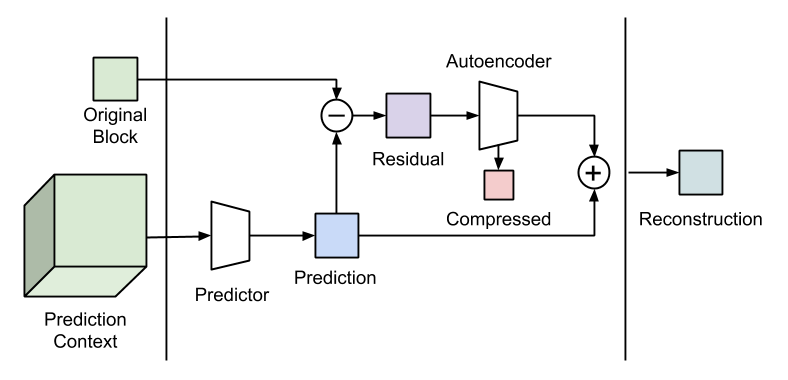
\includegraphics[width=\linewidth]{core_flow}
\end{center}
   \caption{Data flow for the overall network.}
   \label{fig:core}
\end{figure}

One of the key features of modern video codecs is their ability to predict a given block of video based on either blocks from previous frames or already reconstructed blocks within the current frame. Unfortunately if reconstructing a given block depends on previously reconstructed blocks, this means reconstructing a frame block by block must happen entirely in serial. Therefore two different prediction architectures were developed: one where the prediction network only depends on blocks from previous frames, and one where prediction depends on blocks from previous frames as well as the block to the left of the current block, and the block above the current block. For brevity the first prediction scheme will be referred to as the inter-frame prediction scheme and the second will be referred to as the inter-intra-frame prediction scheme (due to its ability to predict from both previous frames and the current frame). The inter-frame scheme can be computed in parallel across all blocks of the video at once, but in the inter-intra-frame scheme, frames must be reconstructed from the upper left block down to the bottom right. In order to keep comparisons between these two prediction methods as equal as possible, they both employed the same network structure, and accepted the same input of the previous $N$ frames. The only difference is that in the inter-intra-frame prediction scheme, the input also contains the current frame, with blocks that have yet to be reconstructed simply set to zero (black).

\begin{figure}[t]
\begin{center}
  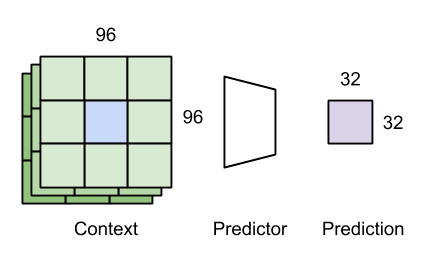
\includegraphics[width=0.8\linewidth]{pred_flow}
\end{center}
   \caption{Input and output of the predictor network.}
   \label{fig:ctx}
\end{figure}


In the interests of reducing computational complexity and limiting the size of the images the prediction networks need to handle, instead of receiving the entire previous frames as input, the predictors instead receive as input a limited surrounding context from previous frames. For a given 32x32 block, the prediction network accepts a 96x96 pixel block from each of the previous $T$ frames, where the 96x96 blocks are centered on the 32x32 block currently being predicted as shown in Figure \ref{fig:ctx}. This allows the predictor to view not only the current block in previous frames, but also all of the neighbor blocks. This limited field of view for the prediction network may pose a problem in scenes with very high movement where the pixels in a given block at frame $i$ were not within the 96x96 view of frame $i - 1$, so the optimal size of the context from previous frames should be an area for further research.

\begin{figure}[t]
\begin{center}
  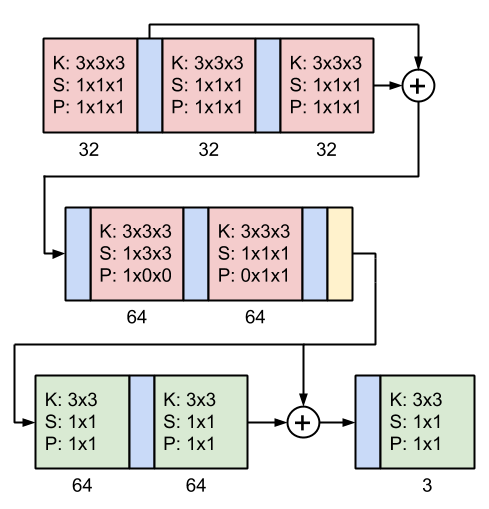
\includegraphics[width=0.8\linewidth]{pred_net}
\end{center}
   \caption{The Predictor network. Red represents 3D convolutions, green represents 2D convolutions, blue represents ReLUs, and yellow represents the squeeze operation to remove the time dimension. K, S, and P stand for kernel size, stride, and padding respectively.}
   \label{fig:pred}
\end{figure}

The predictor network is shown in Figure \ref{fig:pred} and is structured as follows for predicting based on the $3$ previous frames (note that after each convolution in the network, except the final one, is a ReLU nonlinearity that allows the network to model the complex nonlinearities of compression): first the input, of shape Nx3x3x96x96 (where N is the batch size), is passed to a stack of 32 3D convolutions, with stride of 1, padding of 1 and kernel size of 3. The padding ensures that no dimensionality reduction occurs during this step, and since it is a 3D convolution the time dimension of the previous frames is preserved (unlike in a 2D convolution), so the output is Nx32x3x96x96. The data passes through a ResNet \cite{DBLP:journals/corr/HeZRS15} style block of two 3D convolutions with an identity bypass to ensure that gradient is able to reach the first layer. After the ResNet block, the data moves through a layer of 64 3D convolutions with stride of 3 in the height and width dimensions, which compresses the input into Nx64x3x32x32. This prepares the network for the final output shape of 32x32 in the height and width dimensions, and the growth from 32 to 64 layers is intended to ensure that information lost in the spatial reduction can be somewhat preserved with the greater depth. Next the data passes through a 3D convolution that reduces the temporal dimension to size one, allowing the data to be reshaped to Nx64x32x32 (a single image for each batch). Since the temporal dimension has been removed, the data is then passed through another ResNet style block of 2D convolutions (for better gradient flow). Finally a set of three 1x1 2D convolutions reduce the dimension of the data to size Nx3x32x32, giving a prediction image for each batch. 

  Note that since this prediction network is fully convolutional, it can accept arbitrarily sized inputs (although the network was only used on 32x32 blocks), and will simply produce a prediction with one third the width and height of the input. The only exception to this is that changing the temporal dimension (the number of previous frames) requires changing the kernel size of the 3D convolution that reduces the temporal dimension. Otherwise, the temporal dimension would not be size one after the final 3D convolution and the network would be unable to correctly produce a single prediction image. 
  
  Variations on the prediction network were also explored, including a version using Batch Normalization \cite{DBLP:journals/corr/IoffeS15} after every ReLU to improve training and regularization. Other variations included changing the number and size of layers, not using ResNet style blocks, and reducing the temporal dimension before reducing the spatial dimension. The performance of these variations is covered in the results section.

\begin{figure}[t]
\begin{center}
  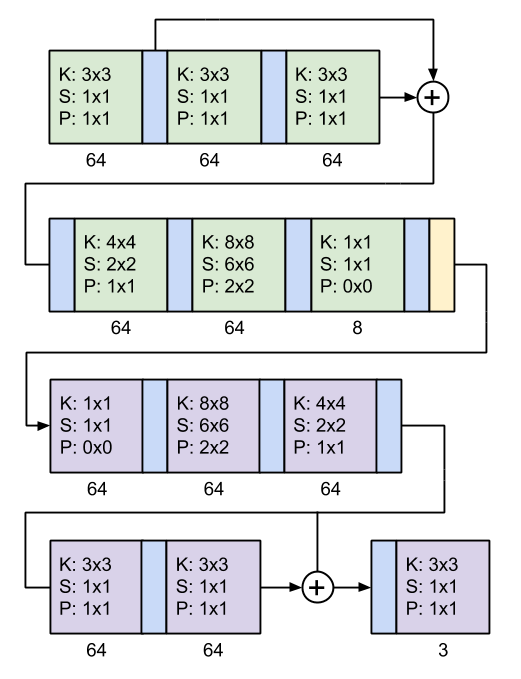
\includegraphics[width=0.8\linewidth]{auto}
\end{center}
   \caption{The Autoencoder network. Green represents 2D convolutions, purple represents 2D transposed convolutions, blue represents ReLUs, and yellow represents an optional quantization operation.}
   \label{fig:auto}
\end{figure}

  After prediction, the other key component of the network is the autoencoder that encodes the residual. Figure \ref{fig:auto} shows the autoencoder, which was designed to reduce a 3x32x32 residual to an 8x3x3 representation (again this network is purely convolutional and could support other input sizes), with support for quantizing the compressed representation into fewer bits for further savings. A version of the autoencoder that contains more layers but similar structure and reduced the input to 4x2x2 was also developed; however this more complex autoencoder qualitatively produced much worse results than simply quantizing the larger residual, so it wasn't explored further. The encoder portion first passes the input into a layer of 64 convolutions with kernel size of 3, and then into a ResNet style block of 2 convolutions, none of which reduce the dimension of the input. Next the input is passed through a series of 2 convolutional layers that use large kernels with strides of 2 and 6 respectively to reduce the spatial dimensions of the input. Finally the encoder passes the input into a 1x1 convolutional layer that reduces the depth from 64 to 8. At this point, the remaining activations can be optionally quantized. Decoding this compressed reconstruction is exactly symmetrical to encoding, except instead of convolutional layers, transposed convolutions are used that up sample the compressed representation back into the original dimensions.

After the prediction network and residual autoencoder are finished, the reconstructed block is passed to the loss function along with the original block. This work experimented with 2 loss functions: per pixel mean squared error (MSE), and Multi Scale Structural Similarity Index (MS-SSIM)\cite{wang2003multiscale}. Although the MSE is very simple mathematically, it is a poor representation of visual quality because it does not take into account preserving the structure of an image, only the per pixel differences, as shown in the following equation where $C$ is the number of channels (3 in this case), $H$ is the height of the image and $W$ is the width of the image:
\[
  MSE(X, \hat{X}) = \frac{1}{CHW} \sum_{c, h, w}\left(X[c, h, w] - \hat{X}[c, h, w]\right)^2
\]

Conversely, MS-SSIM attempts to penalize loss of structural information by accounting for pixel variance at different scales using the standard SSIM calculation:
\[
  SSIM(X, Y) = \frac{(2\mu_X\mu_Y + 0.01)(2\sigma_{XY} + 0.03)}{(\mu_X^2 + \mu_Y^2 + 0.01)(\sigma_X^2 + \sigma_Y^2 + 0.03)}
\]
Where $X$ and $Y$ are two equally sized windows into original image, $\mu$ is the variance of the window, $\sigma$ is the variance and $\sigma_{XY}$ is the covariance of the windows. The final MS-SSIM value is computed by striding the SSIM windows across the images at varying window sizes and computing the average. This results in an output value that ranges from $-1$ to $1$, where 1 is a perfect match between images. Therefore for optimization purposes when using MS-SSIM as part of the loss, the loss is computed as the negative MS-SSIM value. While optimizing for the same metrics as evaluation can be troublesome in video compression due to the lack of a perfect distortion measurement that aligns with human vision, developing a custom loss variance based function to avoid directly optimizing for MS-SSIM was out of the scope for this project.

\section{Experiments \& Results}
The first set of experiments is concerned with comparing the performance of the various network variations described above. When comparing different network variations, the primary metric used was the average per block MS-SSIM achieved by the encoder. Although comparing the MS-SSIM for full frames across different network variations was also used, in most cases there was too much variation across full frame scores to pick an individual network. Additionally, qualitative comparisons of the different networks were also used to catch issues not penalized by the metrics.

The networks were trained as follows: after initial experimentation between RMSProp and Adam as optimizers, little difference was found in performance between the two, so Adam was selected based on default recommendations. Since the training dataset contains a large number of individual blocks, performing hyperparameter optimization across the entire training set was impractical. Therefore a small subset of the training set was selected for hyper parameter optimization, with randomly chosen sets of learning rates and L2 regularization weights selected. Additionally, some experimentation with tuning the number of previous frames to use for the predictor was conducted at the same time; however the memory costs of 3D convolutions made going above 3 previous frames largely impractical. After performing hyper parameter search, 1e-3 was selected as the learning rate and 1e-5 was used as the L2 regularization strength. Although different networks had different optimal hyper parameters, using these numbers gave performance within 0.001 MS-SSIM of more finely tuned results, so hyperparameter optimization was not explored further. Batch size was set to batches of 64 blocks, which is the largest power of two the 4G of VRAM in the GTX 970 used for training could accommodate.

The following network variations were tested:
\begin{enumerate}
  \item
    Reducing spatial dimension before temporal dimension in predictor network, as described in Methods section.
  \item
    Reducing temporal dimension before spatial dimension in predictor network.
  \item
    Same as option 1 except twice as many ResNet style layers in both predictor and autoencoder (batch size reduced to 32 to compensate)
  \item
    Including previously constructed blocks from the current frame in the prediction context. This is the serial approach described in the Methods section.
\end{enumerate}

\begin{figure}[t]
\begin{center}
  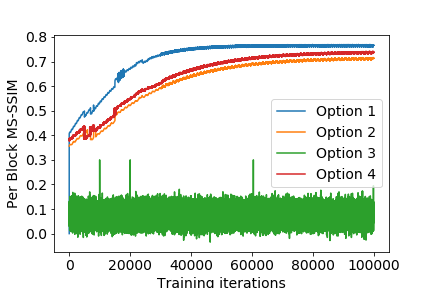
\includegraphics[width=0.8\linewidth]{graph}
\end{center}
   \caption{Training curves of network experiments.}
   \label{fig:plt}
\end{figure}

\begin{table}
  \centering
  \begin{tabular}{cc}
    \toprule
    \thead{Option \#} & \thead{Per Block MS-SSIM}\\
    \midrule
    1 & 0.792\\
    2 & 0.688\\
    3 & 0.122\\
    4 & 0.735\\
    \bottomrule
  \end{tabular}
  \caption{Network experiment results on validation set.}
  \label{tbl:exp}
\end{table}
    
The network variations were compared after training through 3 epochs on a reduced subset of the training set. Although training longer before comparison would have been ideal, it was impractical due to the need to try many different networks with limited compute. After training was complete the networks were evaluated by running on the validation set and measuring the per-block MS-SSIM achieved by each network. Figure \ref{fig:plt} shows the training curves of the four options, and Table \ref{tbl:exp} shows the average MS-SSIM achieved by each strategy on the validation set after training.

As shown by the training curves, option 3 was unable to train effectively, likely due to its increased depth and the need to reduce the batch size to compensate for the increased network size. This option would likely fair better given more training time and a larger batch, but this would require further research. Despite some early instabilities in training across the remaining options, Option 1 performed the best both on the training and the validation set. Interestingly all approaches besides option 3 were able to rapidly reach around 0.5 MS-SSIM, but gains tapered off rapidly around 0.7 MS-SSIM. Despite efforts to reduce learning rates these networks were not able to achieve greater than 0.8 MS-SSIM on average. Additionally, although option 4 performed very well on scenes with low color variation, in many scenes, the color range of the reconstructions was dramatically reduced from the original. This color inaccuracy seems to not have been penalized very heavily by MS-SSIM, so qualitatively option 2 performed better than option 4 despite scoring lower on MS-SSIM.

Due to its higher performance, option 1 was selected for further experimentation. First, Batch Normalization was placed after every ReLU in the network in hopes of reducing overfitting and enabling easier training. One concern was that since many of the training examples contained many adjacent blocks of very similar color (such as the sky), the network would become biased towards predicting low variance monochrome colors. Unfortunately, Batch Normalization significantly reduced the performance of the prediction network. In fact, Batch Normalization seemed to limit the network's ability to reconstruct colors correctly, since although structurally the scene was reconstructed accurately, all reconstructed frames in the network using batch normalization were predisposed to be dominated by the primary color of the scene. Figure \ref{fig:monochrome} shows this effect on a scene from Big Buck Bunny, where the green color of the grass and trees has dominated the entire reconstruction, making the pink clouds green.

\begin{figure}[t]
\begin{center}
  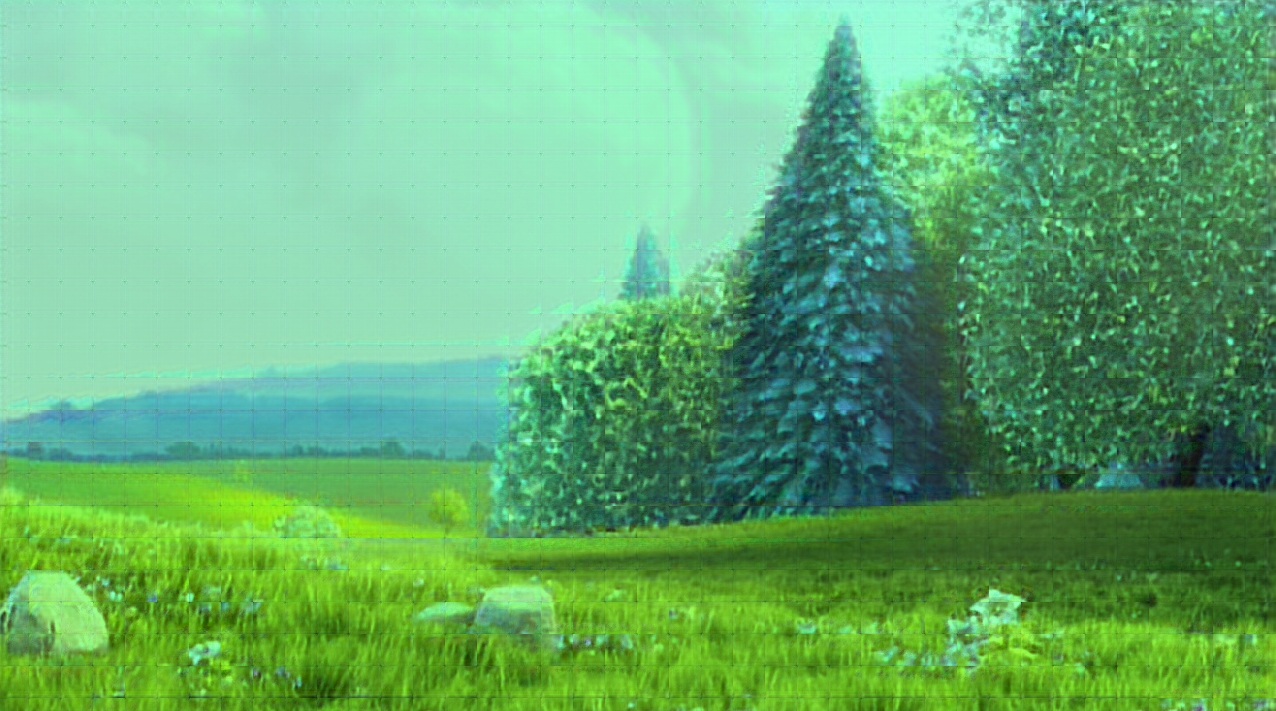
\includegraphics[width=0.8\linewidth]{green}
\end{center}
   \caption{Color distortion seen with Batch Normalization: the clouds should be pink.}
   \label{fig:monochrome}
\end{figure}

Although Batch Normalization was not useful, while debugging the predictor and the autoencoder separately, the idea of also training the two networks separately was tested. Initial experiments to train the predictor and autoencoder both on MS-SSIM were unsuccessful. The predictor in particular seemed unable to accurately reconstruct colors when optimizing for MS-SSIM. Surprisingly, the most successful strategy was to first optimize the predictor to minimize the MSE of its prediction. Minimizing the MSE of the prediction is desirable in order to produce a low magnitude residual for the autoencoder, so the autoencoder would need to encode as little information as possible. Figure \ref{fig:noauto} shows the output of the predictor without any residual correction encoded. Although still relatively visually inaccurate, this image shows that the predictor is capable of largely capturing the overall structure of the scene, admittedly with significant artifacts resulting from block boundaries.
\begin{figure}[t]
\begin{center}
  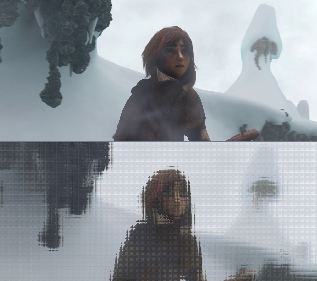
\includegraphics[width=0.8\linewidth]{noauto}
\end{center}
   \caption{The predictor network's reconstruction of a given frame in Sintel, with no residual correction.}
   \label{fig:noauto}
\end{figure}

With the predictor trained down to an average MSE of 0.01 on the validation set, the weights for the predictor were frozen, and the autoencoder was trained to create a residual that maximized the MS-SSIM of the final reconstruction. This process allowed the final network to achieve an average per-block MS-SSIM score of 0.94 on the validation set -- considerably above the 0.8 maximum achieved by training the entire network end to end.

\begin{figure}[t]
\begin{center}
  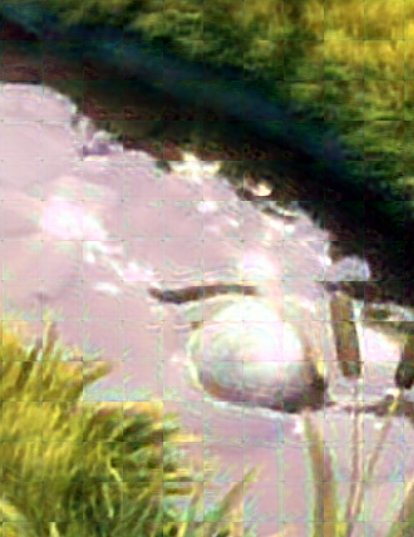
\includegraphics[width=0.4\linewidth]{block}
\end{center}
   \caption{Blocking artifacts present in a reconstructed frame in Big Buck Bunny. Discontinuities are particularly visible in the brightly lit river.}
   \label{fig:block}
\end{figure}

After settling on the separately trained predictor and autoencoder as the best overall strategy, the network's performance was also measured against conventional video codecs as a baseline. The two baselines used were MPEG-2 encoded by FFMpeg and H.264 encoded by FFMpeg using libx264. While MPEG-2 is a very old and outdated codec by modern standards, it contains many of the basic features still employed by modern codecs, so it serves as a reasonable bar for the features a neural network based approach needs to outperform. H.264 is a much more modern codec, widely used in online streaming today. Although many different metrics are available for comparing video compression algorithms, for simplicity MS-SSIM was used as the quantitative measurement of each compression scheme's accuracy. One important note is that the auto-encoder based residual compression described in the previous section does not readily support variable rate compression, which makes the standard video codec metric of a comparison of the area under the rate-distortion curve difficult. While repeatedly encoding successive residuals to support variable rates could be possible, training such an autoencoder was found to be difficult and was abandoned. Instead this work uses quantization of the autoencoder representation to measure distortion at 3 different fixed rates: 1500 kbps (no quantization), 750 kbps and 375 kbps. Additionally, as shown in figure \ref{fig:block} the current block based approach used in this project suffers from serious discontinuities at the block boundaries. Despite trying to ameliorate this issue by computing the MS-SSIM across a wider range than just the current 32x32 block during training, the block artifacts remain persistent. Fortunately, modern video codecs suffer from very similar issues, and have developed post processing filters to remove these block artifacts by smoothing over the discontinuities between blocks. Although an ideal solution would be to develop a neural network based filter that could perform this task and be integrated into the overall system, training on full image frames proved difficult. Instead, for the purposes of gathering data, the deblocking filter from VP8 was used in a final post processing step after reconstructing a frame. The results of full frame compression across the test set at different bit rates are shown in Table \ref{tbl:results}.

\begin{table}
  \centering
  \begin{tabular}{cccc}
    \thead{Codec} & \thead{1500 kbps} & \thead{750 kbps} & \thead{375 kbps}\\
    \midrule
    MPEG-2         & 0.90 & 0.68 & 0.23\\
    H.264          & 0.96 & 0.83 & 0.74\\
    CNN (No deblocking) & 0.68 & 0.59 & 0.55\\
    CNN & 0.84 & 0.80 & 0.79\\
    \bottomrule
  \end{tabular}

  \caption{Full frame average MS-SSIM results on test set.}
  \label{tbl:results}
\end{table}

These results show that the neural network based approach from this project performs quite poorly without a deblocking filter applied. This is not surprising, since MS-SSIM will penalize the variance introduced by the block continuities quite heavily. Fortunately, with a deblocking filter applied, the CNN based approach is quite competitive with MPEG-2 and H.264 at medium to low bitrates (note that the H.264 results are the product of running the encoder in constant bitrate mode, and that other modes would likely give better results, but would not have enabled these fixed rate bitrate experiments). Although the CNN based approach lags behind at higher bitrates, the autoencoder proves to be quite robust to accurately reconstructing a heavily quantized internal representation, which allows the codec to perform well at low bitrates.

One final qualitative issue that should be discussed is the issue of temporal consistency. Rapid noisy changes from frame to frame can be quite visually distracting, but per frame MS-SSIM measurements cannot capture these changes between frames. When operating at low bitrates, the CNN based compression scheme is particularly susceptible to this, as the reconstruction of certain blocks seems to flicker somewhat as quantized residual errors propagate through the autoencoder. Ultimately fixing this issue will require better incorporation temporal consistency into the loss functions for the network.


\section{Conclusion \& Future Work}
The results of this project show that video compression schemes using neural networks are a promising area of research. Given the results generated with limited computational power and time, much better results could be expected from further research into fine tuning the use of 3D CNNs for video compression as well as exploring other similar areas. In particular, given their usefulness in single image compression, recurrent neural network based approaches could offer great benefits by giving the encoder the ability to have fine grained control over what state to read and write from, rather than having a fixed prediction context for each block as in this work.

While the area of frame prediction could undoubtedly be improved given more complex models, the main weak point of the current implementation comes from the autoencoder. In particular, the current model requires a fixed number of bits for each block independent of the accuracy of the prediction or the complexity of the block being represented. This prevents the encoder from devoting more bits to complex parts of a scene, which is a major source of compression savings in modern codecs. Therefore exploring a more flexible model for residual compression would enable significant quality improvements in scenes with large amounts of variety.

Another exciting area for further improvements is the post processing of reconstructed frames. The issue of deblocking already shows the importance of good post processing, and further recent advancements in denoising and super resolution suggest that post processing could significantly increase the perceptual quality of reconstructed frames.

Beyond simple quality and compression ratio improvements, the most significant area requiring further research is the analysis of the performance cost of different compression and reconstruction schemes. Although deeper networks may provide improved visual results, care must be taken to ensure that the resulting networks can eventually be run in real time across a wide variety of hardware to ensure that neural network based video compression schemes are usable in real world applications.

\section{Contributions \& Acknowledgements}
This project used PyTorch 0.4 \cite{pytorch} for constructing and training the network. Additionally the code for SSIM and MS-SSIM in the project is based on the built in implementations within TensorFlow \cite{tensorflow} simply converted to PyTorch code. Video processing (reading in videos and writing out reconstructed videos) is performed with OpenCV \cite{opencv} and FFMPEG \cite{ffmpeg}. The deblocking filter from VP8 uses code taken from the Alfalfa VP8 implementation \cite{alfalfa}.


{\small
\bibliographystyle{ieee}
\bibliography{egbib}
}

\end{document}
